\documentclass{cmc}
\usepackage{makecell}
\usepackage{enumitem}
% \usepackage{subfig}
\begin{document}

\pagestyle{fancy}
\lhead{\textit{\textbf{Computational Motor Control, Spring 2023} \\
    Final project, Project 2, GRADED}} \rhead{Student \\ Names}

\section*{Student names: \ldots (please update)}

% TODO CMC2023: Change the deadline for the project 1
\textit{Instructions: Update this file (or recreate a similar one, e.g.\ in
  Word) to prepare your answers to the questions. Feel free to add text,
  equations and figures as needed. Hand-written notes, e.g.\ for the development
  of equations, can also be included e.g.\ as pictures (from your cell phone or
  from a scanner).  \textbf{\corr{This lab is graded.}} and needs to be
  submitted before the \textbf{\corr{Deadline: Friday 02/06/2023 23:59. For
      project 2, you must submit one final report for all of the following
      exercises separately from the report of project 2. The code of both
      projects can be provided together.}}  Please submit both the source file
  (*.doc/*.tex) and a pdf of your document, as well as all the used and updated
  Python functions in a single zipped file called
  \corr{final\_report\_name1\_name2\_name3.zip} where name\# are the team
  member's last names.  \corr{Please submit only one report per team!}}
\\

%%%%%%%%%%%%%%%%%%%%%%%%%%%%%%%%%%%%%%%%%%%%%%%%%%%%%%%%%%%%%%%%%%%%%%%%%%%%%%%%%%%%%%%%%%%%%%%%%%%%
% \section*{Questions}
\section*{Amphibious Locomotion with Polymander --- CPG Model}\label{sec:exploring-swimming}

In this project you will control a salamander-like robot poymander
 for which you will use Python and the MuJoCo physics
engine. You have an opportunity to use what you've learned until
now to make the robot swim and walk in open and closed loop scenarios.
In order to do this, you should implement a CPG based swimming controller,
similarly to the architecture shown in Figure~\ref{fig:controller-model}.

% TODO CMC2023: Add tegotae paper in the references
% TODO CMC2023: Fix references
The project is based on the research of~\cite{Crespi2013},
~\cite{Karakasiliotis2013},~\cite{ijspeert2007swimming}
and~\cite{thandiackal2021emergence}. It is strongly recommended to
review~\cite{ijspeert2007swimming},~\cite{thandiackal2021emergence} and their
supplementary material provided on the Moodle.
You will be tasked with replicating and studying the
Central Pattern Generator (CPG) network proposed in those papers.

% TODO CMC2023: Change the model to that of ploymander
\begin{figure}[H]
  \centering
  \includegraphics[width=0.9\textwidth]{figures/Polymander_controller_spine.png}
  \caption[Controller model spine]{A double chain of oscillators controlling
    the robot's spine.}\label{fig:controller-model-spine}
\end{figure}

\begin{figure}[H]
  \centering
  \includegraphics[width=0.9\textwidth]{figures/Polymander_controller_leg.png}
  \caption[Controller model limbs]{Single oscillators for each limb}
  \label{fig:controller-model-leg}
\end{figure}

% TODO CMC2023: There is a files.pdf that needs rto generated by gen.py file
% TODO CMC2023: uncomment this when file is generated
\begin{figure}[ht]
  \centering 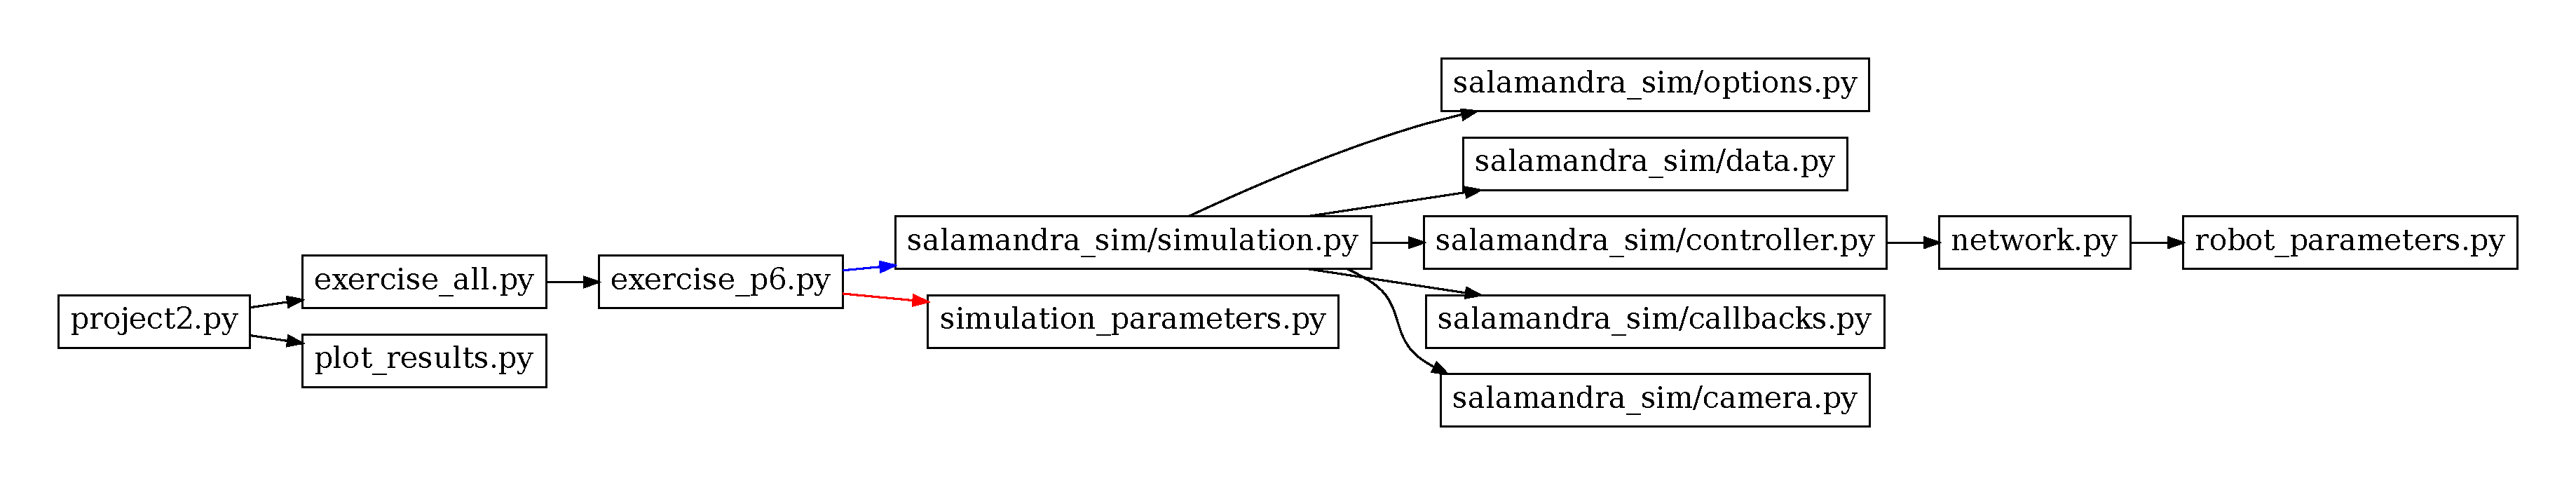
\includegraphics[width=1.0\textwidth]{figures/files}
  \caption{\label{fig:files} Exercise files dependencies. In this lab, you will
    be modifying \fileref{exercise\_\#.py}, \fileref{network.py},
    \fileref{robot\_parameters.py} and \fileref{simulation\_parameters.py}}
\end{figure}

% \newpage

\subsection*{Code organization}\label{subsec:code}

\begin{itemize}
\item \corr{\textbf{project2.py}} --- A convenient file for running the entire
  project. Note you can also run the different exercises in parallel by
  activating \texttt{parallel=True}. \textit{You do not need to modify this
    file.}
\item \corr{\textbf{exercise\_all.py}} --- Another convenient file for running all
  or specified exercises depending on arguments provided. \textit{You do not
    need to modify this file.}
\item \corr{\textbf{network.py}} --- This file contains the different classes and
  functions for the CPG network and the Ordinary Differential Equations
  (ODEs). You can implement the network parameters and the ODEs here. Note that
  some parameters can be obtained from robot\_parameters.py to help you control
  the values.
\item \corr{\textbf{robot\_parameters.py}} --- This file contains the different
  classes and functions for the parameters of the robot, including the CPG
  network parameters. You can implement the network parameters here. Note that
  some parameters can be obtained from the SimulationParameters class in
  \corr{simulation\_parameters.py} and provided in \corr{exercise\_\#.py} to
  help you control the values (refer to example.py).
\item \corr{\textbf{simulation\_parameters.py}} --- This file contains the
  SimulationParameters class and is provided for convenience to send parameters
  to the setup of the network in \corr{network.py::SalamandraNetwork} via the
  robot parameters in \corr{robot\_parameters.py::RobotParameters}. The
  SimulationParameters is also intended to be used for experiment-specific
  parameters for the exercises. All the values provided in SimulationParameters
  are logged for each simulation, so you can also reload these parameters when
  analyzing the results of an experiment.
\item \corr{\textbf{exercise\_\#.py}} --- To be used to implement and answer the
  respective exercise questions. Note that \corr{exercise\_example.py} is
  provided as an example to show how to run a parameter sweep. Note that network
  parameters can be provided here.
\item \corr{\textbf{exercise\_all.py}} --- A convenient file for running different
  exercises depending on arguments. See \corr{\textbf{project1.py}} for an example
  on how to call it. \textit{You do not need to modify this file.}
\item \corr{\textbf{plot\_results.py}} --- Use this file to load and plot the
  results from the simulation. This code runs with the original example provided
  and provides examples on how to collect the data.
\item \corr{\textbf{salamandra\_simulation folder}} --- Contains all the remaining
  scripts for setting up and running the simulation experiments. \textit{You do
    not need to modify any of these file but should still go through them to get
    a better understanding of the code.}

\end{itemize}

% \newpage

\section*{Prerequisites}
The prerequisites for this project are the same as for Project 1.

%%%%%%%%%%%%%%%%%%%%%%%%%%%%%%%%%%%%%%%%%%%%%%%%%%%%%%%%%%%%%%%%%%%%%%%%%%%%%%%%%%%%%%%%%%%%%%%%%%%
\newpage
\section*{Questions}

In the first project, you implemented a network capable to display open loop terrestrial and aquatic locomotion.
You will now extend the network to account
for the presence of exterosensory feedback, contact forces
acting on the limb. You will show how simple contact feedback  (tegotae) affects the limbs and their coordination.
You will expore the open-loop vs closed-loop behaviour for the developed network.
Finally, you will be asked to answer to some open-ended questions regarding possible experimental paradigms.

% %%%%%%%%%%%%%%%%%%%%%%%%%%%%%%%%%%%%%%%%%%%%%%%%%%%%%%%%%%%%%%%%%%%%%%%%%%%%%%%%%%%%%%%%%%%%%%%%%%%%%%%%%%%%%%
% EXERCISE 6 %%%%%%%%%%%%%%%%%%%%%%%%%%%%%%%%%%%%%%%%%%%%%%%%%%%%%%%%%%%%%%%%%%%%%%%%%%%%%%%%%%%%%%%%%%%%%%%%%%%
\newpage
\subsection*{6. Ground Reaction Force feedback}\label{sec:grf-feedback}

In this exercise we will explore how sensory feedback can be used in CPG based controller. Using sensory feedback
in CPG-based controller can impart emergent properties like robustness againts spinal disruptions~\cite{thandiackal2021emergence}
and limb coordination~\cite{owaki2013simple}. In this exercise we will focus on ground reaction forces (grf) and how they can be
used to achieve coordination between limbs as shown by~\cite{owaki2013simple}.

It is recommended to read paper by~\cite{owaki2013simple}, especially section 2. In this paper authors identified
limb oscillator's phase at which the robot's limb is in swing and stance mode.

\begin{itemize}
  \item The swing phase: $ \text{range} \subset (0, \pi) $
  \item The swing phase: $ \text{range} \subset (\pi, 2\pi) $
\end{itemize}

They further identified the phase of the oscillator which corresponds to the middle of stance.
For them this value was  \corr{$ \phi_{stance-mid} = \frac{3\pi}{2} $}. The feedback equation
they used is as follows:

\begin{equation}
  \label{eq:output_fb}
  \dot\phi_i = \omega - \sigma N_i \cos\phi_i
\end{equation}

Where $N_i$ is the grf value from limb i, which governs the oscillator of the same leg. We can
analyse these equation as follows:

\begin{itemize}
  \item Case 1 --- $\phi \subset (0, \frac{\pi}{2})$: This is the swing phase and here $N_i == 0$. \\
        $ \Rightarrow \dot\phi_i = \omega $
  \item Case 2 --- $\phi \subset (\frac{\pi}{2}. \pi)$: This is the swing phase and here $N_i == 0$. \\
        $\Rightarrow \dot\phi_i = \omega $
  \item Case 3 --- $\phi \subset (\pi, \frac{3\pi}{2})$: This is the stance phase and here $N_i > 0$. Plus $\cos\phi_i < 0$ \\
        $ \Rightarrow -\sigma N_i \cos\phi_i$ is positive $\Rightarrow$ \corr{ Feedback in third quadrant accelerates the phase evolution} \\
        Thus when the limb is transitioning from swing to stance it quickly moves towards $\phi_i = \frac{3\pi}{2}$
  \item Case 4 --- $\phi \subset (\frac{3\pi}{2}, 2\pi)$: This is the stance phase and here $N_i > 0$. Plus $\cos\phi_i > 0$ \\
        $ \Rightarrow -\sigma N_i \cos\phi_i$ is negative $\Rightarrow$ \corr{ Feedback in forth quadrant decelerates the phase evolution} \\
        Thus when the limb is transitioning from stance to swing it slowly moves away from $\phi_i = \frac{3\pi}{2}$
\end{itemize}

From the above analysis we can see that the limbs have a tendency to reach the middle of stance and stay there, untill the other limbs
reach the ground. When the other limbs reach the ground, the ground reaction forces \corr{$ N_{\sim i}$ } on those limbs starts to increase
 \corr{$N_{\sim i} > 0$}. Whereas the grf on the limb, \corr{$ N_i $}, start to reduce.
 This ensures that the \corr{deceleration in case 4} is high the limb load \corr{$ N_i $} is high (other limbs are not on ground) and as the limb
 load decreases (other limb have started touching the ground) the effect of slowdown in case 4 due to sensory feedback also reduces. Then the limb $i$
 can transition into the swing phase. Note that the explanation above helps us to understand the basic principle that leads to the interlimb synchronization described in~\cite{owaki2013simple}. However, the mechanisms leading to different patterns of synchronization are complex and are still unknown.

 Next, in this exercise we will apply this feedback for polymander robot and see the effect of the tegotae rule on the simulation of the robot. The phase equation
 for limb oscillators will change as follows:

\begin{equation}
  \label{eq:dphase-grf}
  \dot{\theta}_i = 2 \pi f + \sum_j r_j w_{ij} \sin(\theta_j - \theta_i - \phi_{ij}) + \text{\corr{$f_{N i}$}}
\end{equation}

\corr{
  \begin{equation}
    \label{eq:dphase-feed}
    f_{N i}(N_i, \theta_i) = \sigma N_{i} S(\theta_i)
  \end{equation}
}

Where \corr{ $f_{N i}$ } is the overall feedback due to grf of that limb \corr{($N_i$)}. The function is
governed by weight \corr{$\sigma$}, value of grf \corr{$N_i$} and senstivity function \corr{$S(\theta_i)$}.

Questions:
 \begin{enumerate}
  \item Implement a rigid spine with limb movements. The limbs should be moving as they would in
  previous exercises but with no spine undulation. Explain how this can be achieved.

  \item Plot the limb phase vs ground reaction forces. Find the range of limb phase which corresponds
  to swing and stance. Use thresholding on grf signals to reduce noise. Report the plots achieved.

  \item Identify the \textbf{senstivity function (cos or sin)} which is suited for limb oscillator based on the
  previous plots \& theory of the grf feedback. Identify if the weight ($\sigma$) should be positive or
  negative to generate the same effect as mentioned above.

  \item Implement the feedback and report your observations. Check \corr{network.py} and \corr{controller.py} for the same.
  Set the spine to be rigid.\ Set the body2body weight to 30, and limb2body and body2limb weight to 0. Explain your observations with relevant graphs.

  \item Next, we will add undulating spine and explore the below cases:
  \begin{itemize}
    \item spine undulation, body2body coupling as 10, with no limb to body coupling, no limb to limb coupling
    \item spine undlation, body2body coupling as 10, with limb2body coupling as 30, no limb to limb coupling
    \item spine undlation, body2body coupling as 10, with limb2body coupling as 30, with limb2limb coupling as 10
  \end{itemize}
  Explain your observations with relevant graphs.

  \item Finally, we will observe the differences between open loop and closed loop controller. The following
  four cases should be implemented.
  \begin{itemize}
    \item Open loop \corr{no sensory feedback}: with spine undulation, body2body coupling as 10, with limb2body coupling as 30, no limb to limb coupling
    \item Open loop \corr{no sensory feedback}: with spine undlation, body2body coupling as 10, with limb2body coupling as 30, with limb2limb coupling as 10
    \item Closed loop \corr{with sensory feedback}: with spine undulation, body2body coupling as 10, with limb2body coupling as 30, no limb to limb coupling
    \item Closed loop \corr{with sensory feedback}: with spine undlation, body2body coupling as 10, with limb2body coupling as 30, with limb2limb coupling as 10
  \end{itemize}

  \end{enumerate}

%% -----------------------------SOLUTION EXERCISE 6 ------------------------------

%%%%%%%%%%%%%%%%%%%%%%%%%%%%%%%%%%%%%%%%%%%%%%%%%%%%%%%%%%%%%%%%%%%%%%%%%%%%%%%%%%%%%%%%%%%%%%%%%%%%

\newpage
\subsection*{7. Open question}\label{sec:open_questions}
Choose and answer to one of the following questions.
\begin{enumerate}
\item (Transitions) - Implement the transition between swimming and walking like in exercise 4 in Project 1 without using the GPS data, but using the ground reaction force signal to the feet. Which rule can you think of that will generate the transition?
\item (Local couplings) - So far, you (should) have set global limb to spine coupling as in~\cite{ijspeert2007swimming}. What happens if the connections were set to be local? Implement a local connectivity scheme and test the performance of walking. Can you observe a standing wave during walking?
\item (Scientific proposal) - Propose a scientific question related to the role of sensory feedback in salamander walking and a hypothesis that answers the question. Propose a simulation experiment that could be tested to answer the question. Provide some technical details of this experiment, such as the equations that you would implement to extend the model. Propose a biological experiment that could be designed to confirm the simulation experiment (note: you do not need to implement the suggested proposal).
\item (Swimming with stretch) - Can stretch sensory feedback alone generate swimming coordination when the CPG coupling is removed as in~\cite{thandiackal2021emergence}? Implement the rule proposed in the paper and demonstrate swimming in in the water arena. Show that if the sensory feedback is removed the oscillators cannot synchronize and the animal cannot swim (independently randomize the initial phase of the oscillators).
\end{enumerate}

%%%%%%%%%%%%%%%%%%%%%%%%%%%%%%%%%%%%%%%%%%%%%%%%%%%%%%%%%%%%%%%%%%%%%%%%%%%%%%%%%%%%%%%%%%%%%%%%%%%%

% \newpage

% NOTE: Use this for .bib file instead of listing the \bibitems in the bibliography
% \bibliographystyle{ieetr}
% \bibliography{project1}\label{sec:references}

\begin{thebibliography}{9}

  % Volume, Number, Page, Month, Year
  \bibitem{Crespi2013}
  A. Crespi and K. Karakasiliotis and A. Guignard and A. J. Ijspeert,
  \emph{Salamandra Robotica II:\ An Amphibious Robot to Study Salamander-Like Swimming and Walking Gaits},
  IEEE Transactions on Robotics, Vol. 29, Num. 2, pp.308--320, April 2013,

  \bibitem{Karakasiliotis2013}
  Karakasiliotis, Konstantinos and Schilling, Nadja and Cabelguen, Jean-Marie and Ijspeert, Auke Jan,
  \emph{Where are we in understanding salamander locomotion: biological and robotic perspectives on kinematics},
  Biological Cybernetics, Vol. 107, Num. 5, pp. 529--544, October 2013,

  \bibitem{ijspeert2007swimming}
  Ijspeert, Auke Jan and Crespi, Alessandro and Ryczko, Dimitri and Cabelguen, Jean-Marie,
  \emph{From swimming to walking with a salamander robot driven by a spinal cord model},
  Science, Vol. 315, Num. 5817, pp. 1416--1420, 2007

  \bibitem{thandiackal2021emergence}
  Thandiackal, Robin and Melo, Kamilo and Paez, Laura and Herault, Johann and Kano, Takeshi and Akiyama, Kyoichi and Boyer, Fr{\'e}d{\'e}ric and Ryczko, Dimitri and Ishiguro, Akio and Ijspeert, Auke J,
  \emph{Emergence of robust self-organized undulatory swimming based on local hydrodynamic force sensing},
  Science Robotics, Vol. 6, Num. 56, pp.\ eabf6354, 2021,

  \bibitem{owaki2013simple}
  Owaki, Dai and Kano, Takeshi and Nagasawa, Ko and Tero, Atsushi and Ishiguro, Akio,
  \emph{Simple robot suggests physical interlimb communication is essential for quadruped walking},
  Journal of The Royal Society Interface, Vol. 10, Num. 78, pp. 20120669, 2013,

\end{thebibliography}

% \newpage

% \section*{APPENDIX}
% \label{sec:appendix}

\end{document}

%%% Local Variables:
%%% mode: latex
%%% TeX-master: t
%%% End: